\documentclass[letterpaper, 11pt]{article}
\usepackage{latexsym}
\usepackage{amssymb}
\usepackage{times}
\usepackage{amsmath,amsfonts,amsthm}
\usepackage{graphicx}
\usepackage{amsmath}
\graphicspath{ {pic/} } 
% \oddsidemargin 5mm
\usepackage[letterpaper, margin=1in]{geometry}

\makeatletter
\def\BState{\State\hskip-\ALG@thistlm}
\makeatother


\title{Machine Learning: Data to Models \\Assignment 2b}
\author{Qun Gao, JHED ID qgao6: \\Li-Yi Lin, JHED ID: llin34}
\date{}

\begin{document}

\maketitle
\noindent \Large \textbf{3.1 Learning: Parameter Estimation [50 points]}\\
\large \textbf{3.1.4 Program overview: [40 points]}\\
The program can be divided into following parts:
\begin{enumerate}
\item Parse the network data: the program reads all the variables and their values from the network file and also keeps the relationship between variables. Since we use parameter sharing method, for the variables in an example with the same time stamp, we ignore the time stamp. For those with different time stamps in an example, we use $T0$ and $T1$ to represent the time sequence.
\item Construct the counting table: the program then constructs all the possible outcome of the events and add one to each of them.
\item Do the counting: the program reads all the examples and also parses the examples by converting them to the parameter sharing format. For the position parameter sharing, the program will determine how many steps, 0 or 1, the robot moves in an example. It then adds one to the corresponding count. For each example, if we did not have the observation for some observable objects, it will add one to the count of the event that (observable object=No given other variables).
\item Output the CPD: When outputing the result, the program will loop all the possible outcomes and maps the parameter sharing format to the final output format and find its probability, its count divided by the total number of counts that belong to the same CPD.
\end{enumerate}
\large \textbf{3.1.5 Analytical Questions [10 points]}\\
1. [3 points] 
Since model with large amount of parameters could cause overfitting so sharing parameters in the model reduced a lot of parameters and thus reducing the effects of overfitting. In our assignment the sample size isn't large enough to well estimate every parameter if we don't share parameters and consider all possible ones. It will cause overfitting and some parameters couldn't be estimated with current samples.\\
\\
2. [3 points]
If we consider the robot walking outdoor, and there are two possible road conditions: flat ground and hill, we reasonablely assume that the probability of  the robot staying at the same place at the next time on the hill is sightly larger than it on the flat ground. In this case we should consider the difference of the parameters in different positions, i.e., we couldn't share parameters for the probability of the robot walking on the flat ground and on the hill. And we should use an explicit parameterization.\\
\\
3. [4 points]
We can consider the following: we cluster the different conditions related to time or position (e.g. flat ground and hill for robot walking outdoor) and share parameters within each cluster. For different clusters we assign different parameters. For instance, in the previous question, we consider the probability of the robot staying at the same place at the next time on the hill is different from it on the flat ground, i.e. we perform two different parameters. But we assume that the probability of the robot moving one step on the flat ground stays the same for different positions. In this new model, we relatively learned unique values for all CPT entries but since the model shared parameters within clusters it still reduced overfitting. This method is more advantaged because it reduced overfitting and is more robust than the approach of sharing parameters all the way.\\
\\
\noindent \Large \textbf{3.2 Inference [90 points]}\\
\large \textbf{3.2.1 Analytical Questions: Clique Tree [20 points]}\\
1. [2 points]\\
Step 1: 
Draw the Bayesian network of a given model. And convert this directed graph into undirected graph by "marrying" the parents of each node and converting directed edges to undirected ones.\\
Step 2: 
Create a chordal graph by triangulation.\\
Step 3:
Find all maximal cliques in the chordal graph and form a cluster graph over these cliques by connecting cliques with common variables and assign weights  to these edges with the number of variables they have in common.\\
Step 4:
Find the maximal spanning tree over this cluster graph and use it as the clique tree.\\
\\
2. [2 points]
If a variable $S$ is in both cluster $C_i$ and $C_j$ in the clique tree, then it will in each cluster that is in the path from $C_i$ to $C_j$. For example, 
PositionRow\_1 is in cluster $C_1=$ (Action\_0, PositionCol\_0,PositionRow\_1,PositionCol\_1) and cluster $C_2=$ (ObserveLandmark2\_E\_1,PositionRow\_1, PositionCol\_1), then it will in each cluster in the path $C_1-C_3-C_2$, where $C_3=$ (Action\_1, PositionRow\_1, PositionCol\_1,PositionRow\_2). So this implies that the running intersection property holds.\\
\\
3. [2 points]
We wrote a Python script to generate the clique tree files. We found that the clique tree for different parameter settings have the same pattern, i.e. \\
For the clusters, the pattern is:\\
$Action\_(n),PositionRow\_(n),PositionCol\_(n),PositionRow\_(n+1)$\\
$Action\_(n),PositionCol\_(n),PositionRow\_(n+1),PositionCol\_(n+1)$\\
$ObserveWall\_(Direction)\_(n),PositionRow\_(n),PositionCol\_(n)$\\
$ObserveLandmark(L)\_(Direction)\_(n),PositionRow\_(n),PositionCol\_(n)$\\
where\\ 
$(n)$ is the time stamp, \\
$(Direction)$ is "N", "S", "E", and "W", and \\
$(L)$ is the landmark number.\\
And in the last line of the clusters, we add $Aciton\_N$, where $N$ is the largest time stamp.\\

\noindent
For the edges, the pattern is:\\
$Action\_(n),PositionRow\_(n),PositionCol\_(n),PositionRow\_(n+1)$\\
connects with\\
$Action\_(n),PositionCol\_(n),PositionRow\_(n+1),PositionCol\_(n+1)$, \\
$ObserveWall\_(Direction)\_(n),PositionRow\_(n),PositionCol\_(n)$, and\\
$ObserveLandmark(L)\_(Direction)\_(n),PositionRow\_(n),PositionCol\_(n)$\\

\noindent
and before adding one to $(n)$, \\
$Action\_(n),PositionCol\_(n),PositionRow\_(n+1),PositionCol\_(n+1)$\\ 
will connect with\\ 
$Action\_(n+1),PositionRow\_(n+1),PositionCol\_(n+1),PositionRow\_(n+2)$\\
\\
4. [4 points]
If we simply marginalize over a joint CPT to compute the distribution of the final position at time T, the computational complexity is $O(M^TN^T4^T2^{12T}) = O((2^{14}MN)^T)$. If we use message passing in our clique tree, the total number of message passaging is $2(T-1)-1 = 2T-3$. For each massage passing, the operations takes time $4M^2N$ or $4MN^2$. Let $M < N$, then the total computational complexity is $O((2T-3)MN^2) = O(TMN^2)$.\\
\\
5. (a) [7 points]
We could modify the clique tree by holding the query variables at time 5 in each clique in the path from clique at time 5 to clique at time 15 (as shown in the figure 1) when constructing the clique tree.

\begin{figure}[hbtp]
\centering
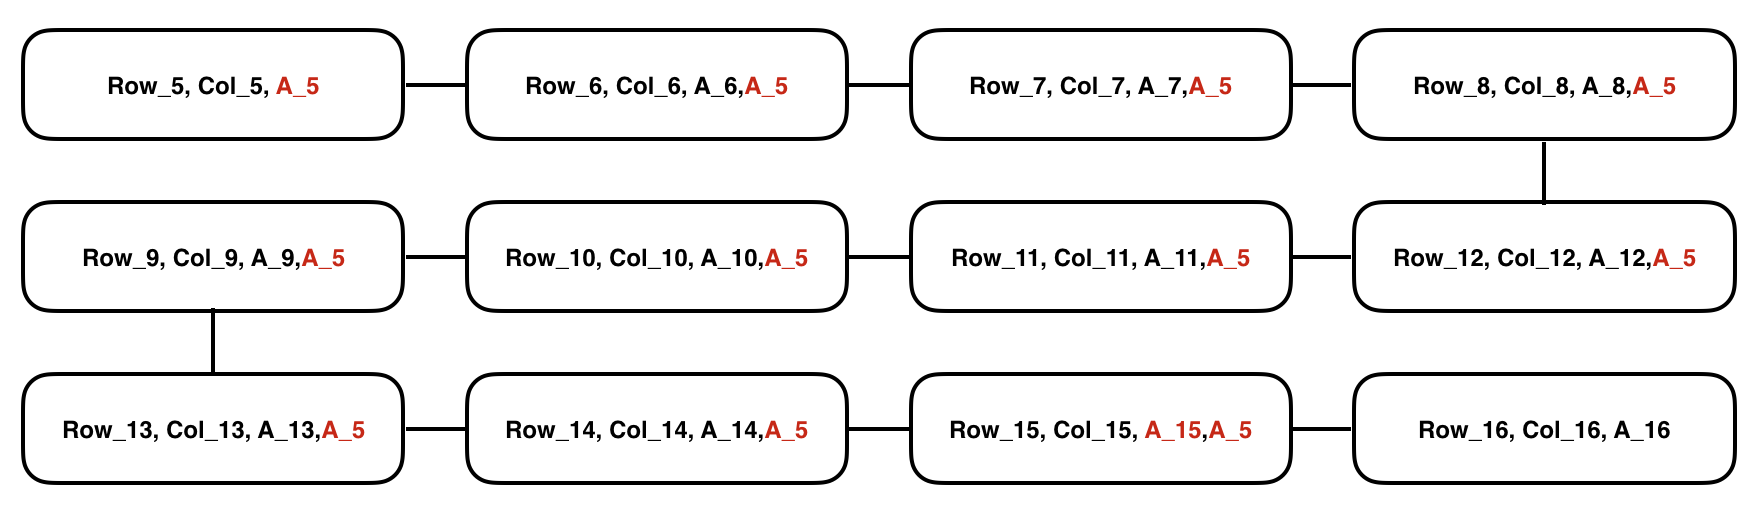
\includegraphics[scale=0.5]{clique.png}
\caption{example of method for modifying the clique tree}
\end{figure}

(b) [3 points]
Because if we just use the potential of two different clusters containing the query variables, we can't get the joint probability that contains all of the query variables for marginalization.









\end{document}